\chapter{引言（示例章节）}
\label{chap:introduction}

本章介绍研究报告的基本结构和研究背景的撰写方法。

\section{研究背景}
研究背景部分应当说明研究工作的宏观背景和微观背景。
宏观背景可从行业发展趋势、国家政策导向等方面展开。
微观背景则应聚焦于具体研究领域的发展现状和存在问题。

例如，随着我国经济社会的快速发展，相关领域面临着一系列新的挑战和机遇。
这些挑战和机遇为本研究提供了重要的研究背景和研究动机\cite{example2023}。

\section{研究现状}
研究现状部分应当系统梳理国内外相关领域的研究进展。

\subsection{国外研究现状}
国外学者在该领域开展了大量研究工作。Smith等\cite{smith2022}提出了...
Johnson\cite{johnson2021}通过实验研究发现...

\subsection{国内研究现状}
国内学者也进行了相关研究。张三等\cite{zhang2020}研究了...
李四\cite{li2019}从理论角度分析了...

\subsection{研究现状总结}
综合国内外研究现状，可以发现：
（1）现有研究主要集中在...方面；
（2）在...方面的研究相对较少；
（3）存在...问题亟待解决。

\section{研究内容与目标}
\subsection{研究内容}
本报告主要研究内容包括：
\begin{enumerate}
    \item 第一项研究内容：简要说明研究内容的具体描述。
    \item 第二项研究内容：简要说明研究内容的具体描述。
    \item 第三项研究内容：简要说明研究内容的具体描述。
\end{enumerate}

\subsection{研究目标}
本研究的主要目标包括：
\begin{itemize}
    \item 目标一：简要描述研究目标。
    \item 目标二：简要描述研究目标。
    \item 目标三：简要描述研究目标。
\end{itemize}

\section{研究方法与技术路线}
本研究采用的主要研究方法包括理论分析、数值模拟和实验研究等。
技术路线如图\ref{fig:tech_route}所示。

\begin{figure}[htbp]
    \centering
    % 请替换为实际的流程图文件
    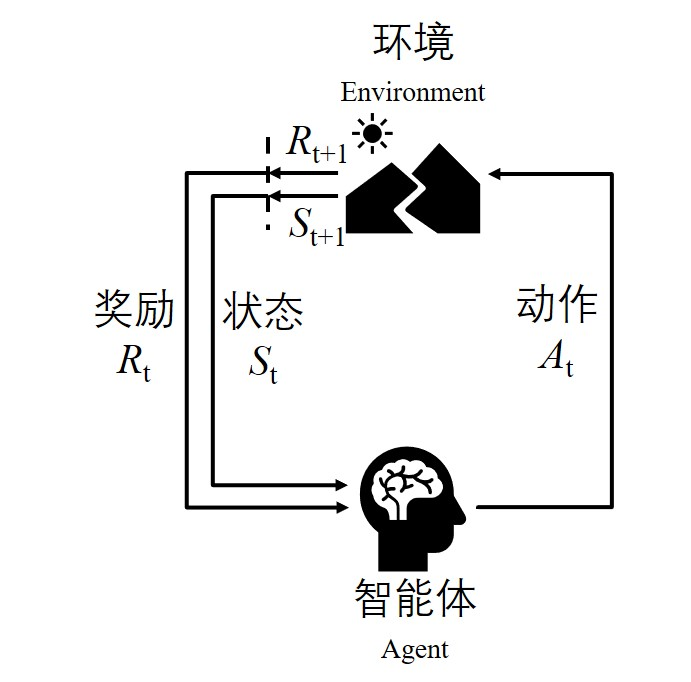
\includegraphics[width=0.8\textwidth]{figures/RL_Framework.jpg}
    \caption{研究技术路线示意图（示例）}
    \label{fig:tech_route}
\end{figure}

\section{报告结构安排}
本报告共分为六章，各章主要内容如下：

第一章为引言，介绍研究背景、研究现状和研究内容等。

第二章为研究方法示例章，展示图表、公式、算法等格式的使用方法。

第三章为实验研究示例章，展示表格、多图排版等格式的使用方法。

第四章为数值分析示例章，展示参考文献引用等格式的使用方法。

第五章为结果讨论示例章，展示结果展示格式。

第六章为结论与展望，总结研究成果并展望未来研究方向。